\documentclass[12pt, a4paper]{report}

\usepackage[czech]{babel}
\usepackage[IL2]{fontenc}
\usepackage[utf8]{inputenc}
\usepackage{lmodern}  % lepší kvalita PDF

\usepackage[a4paper,top=3cm,bottom=3cm,left=3cm,right=3cm,marginparwidth=1.75cm]{geometry}

\usepackage{graphicx}
\usepackage{titling}
\usepackage[colorlinks=true, allcolors=black]{hyperref}
\usepackage{url}
\usepackage{enumitem}

% formátování zdrojového kódu
\usepackage{listings}
\usepackage{color}

\definecolor{dkgreen}{rgb}{0,0.6,0}
\definecolor{gray}{rgb}{0.5,0.5,0.5}
\definecolor{mauve}{rgb}{0.58,0,0.82}

\lstset{frame=tb,
	language=C,
	aboveskip=3mm,
	belowskip=3mm,
	showstringspaces=false,
	columns=flexible,
	basicstyle={\small\ttfamily},
	numbers=none,
	numberstyle=\tiny\color{gray},
	keywordstyle=\color{blue},
	commentstyle=\color{dkgreen},
	stringstyle=\color{mauve},
	breaklines=true,
	breakatwhitespace=true,
	tabsize=4,
	extendedchars=true,
	literate=%
	{á}{{\'a}}1
	{č}{{\v{c}}}1
	{ď}{{\v{d}}}1
	{é}{{\'e}}1
	{ě}{{\v{e}}}1
	{í}{{\'i}}1
	{ň}{{\v{n}}}1
	{ó}{{\'o}}1
	{ř}{{\v{r}}}1
	{š}{{\v{s}}}1
	{ť}{{\v{t}}}1
	{ú}{{\'u}}1
	{ů}{{\r{u}}}1
	{ý}{{\'y}}1
	{ž}{{\v{z}}}1
	{Á}{{\'A}}1
	{Č}{{\v{C}}}1
	{Ď}{{\v{D}}}1
	{É}{{\'E}}1
	{Ě}{{\v{E}}}1
	{Í}{{\'I}}1
	{Ň}{{\v{N}}}1
	{Ó}{{\'O}}1
	{Ř}{{\v{R}}}1
	{Š}{{\v{S}}}1
	{Ť}{{\v{T}}}1
	{Ú}{{\'U}}1
	{Ů}{{\r{U}}}1
	{Ý}{{\'Y}}1
	{Ž}{{\v{Z}}}1
}
\lstset{language=C}

% vlastní příkazy
\newcommand{\lt}{\textless}
\newcommand{\gt}{\textgreater}

\title{Interpret podmnožiny jazyka Lisp}
\def \thesubtitle {Semestrální práce z předmětu KIV/PC}
\author{Patrik Harag}
\def \theauthoremail {harag@students.zcu.cz}
\def \theauthorid {(A15B0034P)}

\begin{document}

% titulní strana
\begin{titlepage}
	\begin{figure}
		
\includegraphics[height=50mm]{img-fav-logo}
	\end{figure}
	
	\centering
	{\large \hspace{1mm} \par} % tady musí být nějaký text jinak nefunguje vertikální odsazení
	\vspace{15ex}
	
	{\scshape\Large \thesubtitle \par}
	\vspace{1.5ex}
	{\huge\bfseries \thetitle \par}
	\vspace{2ex}
	{\Large\itshape \theauthor \par}
	\vspace{2ex}
	{\texttt{\theauthoremail} \par}
	\vspace{1ex}
	{\texttt{\theauthorid} \par}
	
	\vfill
	
	{\large \today \par}
\end{titlepage}

% strana s obsahem
\setcounter{page}{0} 
\tableofcontents
\thispagestyle{empty}


\chapter{Zadání}
Naprogramujte v ANSI C přenositelnou konzolovou aplikaci, která bude fungovat jako jednoduchý interpret podmnožiny funkcionálního programovacího jazyka Lisp. Vstupem aplikace bude seznam příkazů v jazyce Lisp. Výstupem je pak odpovídající seznam výsledků vyhodnocení každého výrazu.\\

\noindent
Program se bude spouštět příkazem \verb|lisp.exe| [\lt\textit{vstupní-soubor}\gt].\\Symbol \lt\textit{vstupní-soubor}\gt \vspace{1pt} zastupuje nepovinný parametr – název vstupního souboru se seznamem výrazů v jazyce Lisp.
Není-li první parametr uveden, program bude fungovat v interaktivním módu, kdy se příkazy budou provádět přímo zadáním z konzole do interpretu.\\

\noindent
Vámi vyvinutý program tedy bude vykonávat následující činnosti:
\begin{enumerate}
	\item Při spuštění bez parametru bude čekat na vstup od uživatele. Zadaný výraz vyhodnotí a bude vyžadovat další vstup, dokud nebude uveden výraz \verb|(quit)|.
	\item Při spuštění s parametrem načte zadaný vstupní soubor, každý výraz v něm uvedený vypíše na obrazovku, okamžitě vyhodnotí a výsledek vypíše na obrazovku. Po zpracování posledního výrazu dojde k ukončení programu. Proto nemusí být jako poslední výraz uveden výraz \verb|(quit)|. Na jedné řádce v souboru může být uvedeno více samostatných výrazů a program je musí být schopen správně zpracovat.
\end{enumerate}

\noindent
Váš program může být během testování spuštěn například takto:\\

\noindent
\verb|lisp.exe test.lisp|\\

\noindent
Celé zadání je dostupné na adrese:

\mbox{\url{http://www.kiv.zcu.cz/studies/predmety/pc/doc/work/sw2016-01.pdf}}


\chapter{Analýza}
\section{Charakteristika jazyka Lisp}
Program v jazyce Lisp\footnote{Většinou bývá názvem Lisp označována celá rodina jazyků, přičemž jednotlivé dialekty se od sebe mohou výrazně lišit. Zadání neuvádí žádný konkrétní dialekt nebo verzi, pouze přikládá odkaz na online interpret jazyka \emph{Common Lisp} s názvem \emph{JSCL}.} je složen z takzvaných \emph{s-výrazů}\footnote{Termín \emph{s-výraz} (\emph{s-expression}) bude používán pouze ve smyslu způsobu zápisu syntaxe, nikoli ve smyslu způsobu reprezentace dat ve stromové struktuře.} neboli seznamů ve tvaru

\vspace{5pt}
\centerline{$(\lt\emph{funkce}\gt \lt\emph{argument-1}\gt \lt\emph{argument-2}\gt \dots),$}
\vspace{5pt}
\noindent
kde na prvním místě je název funkce a na dalších její argumenty. Prvkem s-výrazu může být opět s-výraz. Všechny funkce a syntaktické konstrukty jazyka mají identický zápis. Zdrojový kód v jazyce Lisp má stejnou strukturu jako jeho \emph{abstraktní syntaktický strom} (\emph{AST}) – tato vlastnost se nazývá \emph{homoikonicita}.

Programovací jazyk Lisp je vybaven takzvanou smyčkou \emph{REPL} (\emph{Read-Evaluate-Print-Loop}), interaktivním prostředím, v němž je možné zapisovat jednotlivé výrazy, které jsou ihned vykonány a jejichž výsledek je vypsán na standardní výstup. Naším úkolem bude podobnou smyčku vytvořit.

\section{Návrh parseru}
Díky výše uvedeným vlastnostem je tvorba parseru, oproti konvenčním jazykům, relativně jednoduchá.
V první fázi bude vstup rozdělen na jednotlivé tokeny. Token může být závorka nebo libovolné slovo, které oddělují bílé znaky nebo závorky.
Z~tokenů se následně sestaví abstraktní syntaktický strom, neboli soustava s-výrazů.

Tvorbu parseru však zkomplikuje speciální zápis funkce \emph{QUOTE}, znak \uv{\emph{'}}, který se přepisuje jako:\\
\centerline{$\emph{'}\lt\textit{výraz}\gt \rightarrow (\emph{QUOTE}$ $\lt\textit{výraz}\gt)$}

\vspace{5pt}
Jako vhodné řešení se nabízí provést tuto transformaci až po sestavení abstraktního syntaktického stromu s tím, že parser \uv{nebude vědět} nic o tomto speciálním zápisu a zachová si tak svoji jednoduchost. Bude se tak v podstatě jednat o makro.

\section{Návrh interpretu}

\paragraph{Datové typy}
Jazyk bude podporovat několik datových typů -- minimálně logický typ, celé číslo, symbol a seznam.
Hodnoty budou ukládány do generické struktury, která bude obsahovat číslo určující typ hodnoty a ukazatel na hodnotu.

\paragraph{Paměť}
Uživatelské proměnné je nutné mezi jednotlivými vyhodnocovanými výrazy někam ukládat. Stejně tak je nutné někam uložit seznam funkcí. Je zde možnost tyto struktury spojit do jedné.

\paragraph{Výjimky}
Při implementaci interpretu bude nutné od začátku počítat s nutností nějakým způsobem zpracovávat výjimky. K výjimce může dojít i uvnitř vnořených forem, je tedy potřeba implementovat jejich propagaci.

\paragraph{Vlastnosti funkcí}
V některých dialektech jazyka Lisp je funkce takzvaný \emph{first-class citizen}. To znamená, že je s funkcí nakládáno, jako s jakýmkoliv jiným objektem, tedy může být předána jako argument funkce, uložena do proměnné nebo vrácena jinou funkcí.
Jiné implementace zacházejí s funkcemi odlišně, než s jinými hodnotami.
V~naší implementaci bude funkce \emph{first-class citizen}, protože to považuji za důležitou vlastnost, která do jazyka přinese jednotnost a jednoduchost.


\chapter{Implementace}

\section{Postup interpretace}
Významnou roli hraje soubor \emph{repl.c}, který spojuje ostatní moduly a řídí tak proces interpretace.

Vstupní řetězec, načtený z konzole nebo ze souboru, je nejprve rozdělen na jednotlivé tokeny (zajišťuje \emph{lexer.c}), z nich je následně sestaven AST a aplikováno makro \emph{QUOTE} (\emph{reader.c}). Kompletní AST je poté předán k vyhodnocení (\emph{interpreter.c}) a~výsledek je vypsán do konzole (\emph{console.c}).

\subsection{Načítání ze souboru}
Při načítání ze souboru se znaky ukládají do vyrovnávací paměti, dokud není načten celý výraz. Následně je načtený výraz vypsán do konzole, standardním způsobem vyhodnocen a výsledek vypsán.

Interpret by si sice dokázal poradit i s celým zdrojovým kódem najednou (REPL standardně podporuje i více výrazů na jednom řádku), nicméně už bychom z něj nedostali vstupní řetězce, které potřebujeme jednotlivě vypsat do konzole.

\section{Datové typy}
Interpret podporuje následující datové typy:
\begin{itemize}
	\item Logická hodnota
	\item Celé číslo
	\item Symbol
	\item Seznam
	\item Funkce
	\item Speciální forma 
	\item Výjimka
\end{itemize}
Hodnoty všech výše uvedených datových typů jsou ukládány do jedné generické struktury s názvem \emph{Value}.

\begin{lstlisting}
typedef struct _Value {
    int type;  /* konstanta určující typ hodnoty */
    void *pointer;  /* pointer na hodnotu */
} Value;
\end{lstlisting}

Funkce pro práci s hodnotami, příslušné struktury a konstanty jsou uloženy v~souborech \emph{types.h} a \emph{types.c}.

\subsection{Logické hodnoty}
Logické hodnoty jsou vnitřně reprezentovány stejně jako celá čísla. Toto řešení bylo použito zejména kvůli konzistenci.

\subsection{Celá čísla}
Celá čísla jsou reprezentovány datovým typem \emph{int} jazyka C.
Do struktury \emph{Value} se tedy uloží pointer na \emph{int}. 

\subsection{Symboly}
Symboly slouží primárně k pojmenování hodnot prostřednictvím funkce \emph{SET}. Vnitřně jsou reprezentovány textovým řetězcem.

\subsection{Seznamy}
V seznamu je možné uchovávat hodnoty libovolného typu. Seznam je implementován polem:

\begin{lstlisting}
typedef struct _ValueList {
	int length;
	Value **values;
} ValueList;
\end{lstlisting}
Do struktury \emph{Value} se uloží pointer na strukturu \emph{ValueList}.

\subsection{Funkce}
Funkce jsou ukládány jako struktury, které obsahují pointer na zdrojovou funkci.

Pointer na funkci nemůže být použit (uložen do struktury \emph{Value}) přímo, protože v ANSI C není možné kombinovat datové pointery s pointery ukazujícími na funkce. Jinými slovy pointer na funkci nelze přetypovat na \verb|void *|.

Zdrojové funkce se nestarají o uvolňování paměti předaných parametrů.
Zároveň také musí vracet vždy novou hodnotu, nikdy tedy nesmí vrátit hodnotu předanou parametrem.
Tyto podmínky jsou dány systémem, jakým se v programu pracuje s~dynamickou pamětí.

\pagebreak[2]

\noindent
Typy pro práci s funkcemi:
\begin{lstlisting}
/* pointer na funkci */
typedef Value * (*Function) (int argc, Value **argv);

/* struktura pro zabalení pointeru na funkci */
typedef struct _FunctionWrapper {
    Function function;
} FunctionWrapper;
\end{lstlisting}

\vspace{2ex}
\noindent
Příklad implementace funkce \emph{LENGTH} (\emph{built-in\_list.c}):
\begin{lstlisting}
Value * func_list_length(int argc, Value **argv) {
    if (argc < 1)
        return value_exception(MSG_TOO_FEW_ARGUMENTS);

    if (argv[0]->type != TYPE_LIST)
        return value_exception(MSG_WRONG_TYPE);

    return value_integer(as_list(argv[0])->length);
}
\end{lstlisting}

\subsection{Speciální formy}
Speciální formy jsou prostředkem, kterým se zavádí jazykové konstrukce (smyčky, podmíněné příkazy, částečně vyhodnocované formy atd.).

Podobají se funkcím, ale jsou vyhodnocovány odlišným způsobem. Na rozdíl od běžných funkcí nejsou jejich argumenty před předáním vyhodnoceny. Speciální formy tedy při vyhodnocení dostávají, místo seznamu hodnot, seznam s-výrazů.

Stejně jako u \uv{klasických} funkcí jsou pointery speciálních forem zabalovány do struktur. Funkce implementující speciální formy se také nestarají o uvolňování předaných parametrů.

\vspace{2ex}
\noindent
Typy pro práci se speciálními formami:\begin{lstlisting}
/* pointer na speciální formu */
typedef Value * (*SpecialForm) (int count, SExpression **exprs);

/* struktura pro zabalení pointeru na funkci */
typedef struct _SpecialFormWrapper {
    SpecialForm function;
} SpecialFormWrapper;
\end{lstlisting}

\subsection{Výjimky}
Výjimky jsou implementovány stejně jako jiné běžné hodnoty. Obsahem výjimky je řetězec obsahující chybovou zprávu.

Pokud některá funkce vrátí výjimku, interpretr ji zachytí, případně přeruší další vyhodnocování a výjimku propaguje do vyšší úrovně.

\section{Globální paměť}
Díky jednotnému typovému systému mohou být všechny funkce, speciální formy i~uživatelské proměnné uložené v jedné datové struktuře. Tuto strukturu budeme nazývat, jak je zvykem, halda. Halda umožňuje vytvořit proměnné i konstanty. Pokud se uživatel pokusí konstantu předefinovat, bude mu v tom zabráněno.

Pro jednoduchost jsou logické literály \emph{T} a \emph{NIL} ve skutečnosti uloženy na haldě jako konstanty, ale pro uživatele v tom není žádný rozdíl.

Halda je definována v souboru \emph{heap.h} a implementovaná v \emph{heap.c}.


\chapter{Uživatelská příručka}

\section{Sestavení}
Pro snadné sestavení je připraven \emph{Makefile}, který funguje na operačním systému Linux a v případě správné konfigurace i na Windows. Sestavení se provede po zavolání příkazu \verb|make| v kořenovém adresáři. Předpokladem je nainstalovaný \emph{GCC}, popřípadě \emph{MinGW} (Windows) a nástroj \emph{make}.

Pro operační systém Windows je připraven ještě poněkud typičtější \emph{Makefile.win}. Překlad je obvykle možné provést příkazem \verb|make -f Makefile.win|. Předpokladem je nainstalovaný překladač \emph{Microsoft C/C++} a nástroj \emph{make}.

Příkazy pro přeložení se mohou lišit podle použitého překladače a nastavení.

\section{Spuštění}
Program je možné spustit dvěma způsoby:

\begin{itemize}
	\item \verb|lisp.exe|
	
	Program bude fungovat v interaktivním módu, kdy se příkazy budou provádět přímo zadáním z konzole do interpretu. Příklad použití ukazuje Obrázek \ref{fig:repl}
	
	\item \verb|lisp.exe <vstupní-soubor>|
	
	Při spuštění s parametrem načte zadaný vstupní soubor, každý výraz v něm uvedený vypíše na obrazovku, okamžitě vyhodnotí a výsledek vypíše na obrazovku. Po zpracování posledního výrazu dojde k ukončení programu.
\end{itemize}

\begin{figure}[h]
	\centering
	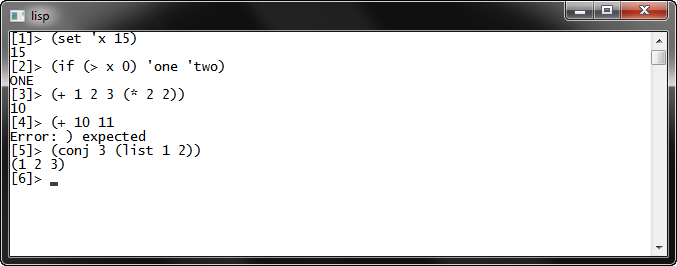
\includegraphics[width=0.9\linewidth]{img-repl}
	\caption{Ukázka práce v interaktivním módu (REPL)}
	\label{fig:repl}
\end{figure}

Na jedné řádce v souboru může být uvedeno více samostatných výrazů. V takovém případě se vyhodnotí a vypíší všechny.

\pagebreak
\section{Seznam funkcí}

\setlength{\tabcolsep}{0.5em} % for the horizontal padding
{\renewcommand{\arraystretch}{1.5}% for the vertical padding

\begin{table}[ht]
	\caption{Aritmetické funkce.}
	\centering
	\vspace{5pt}
	
	\begin{tabular}{||c p{11cm}||} 
		\hline
		Název funkce & Popis \\ %[0.5ex] 
		\hline\hline
		\verb|+| & Sečte prvky a vrátí celočíselný výsledek. \\ 
		\hline
		\verb|-| & Odečte prvky zleva doprava a vrátí celočíselný výsledek. \\
		\hline
		\verb|*| & Vynásobí prvky a vrátí celočíselný výsledek. \\ 
		\hline
		\verb|/| & Vydělí od sebe prvky zleva doprava a vrátí celočíselný výsledek. Prováděno bude vždy jen celočíselné dělení. \\
		\hline
	\end{tabular}
\end{table}

\begin{table}[ht]
	\caption{Porovnávací funkce.}
	\centering
	\vspace{5pt}
	
	\begin{tabular}{||c p{11cm}||} 
		\hline
		Název funkce & Popis \\ %[0.5ex] 
		\hline\hline
		\verb|=| & Porovná sousední prvky na shodu a výsledkem je \verb|T| nebo \verb|NIL|. Výsledek je dán logickým součinem všech porovnání. \\
		\hline
		\verb|/=| & Porovná sousední prvky na neshodu a výsledkem je \verb|T| nebo \verb|NIL|. Výsledek je dán logickým součinem všech porovnání. \\ 
		\hline
		\verb|<| & Porovná sousední prvky operátorem \verb|<| (menší než) a vrátí výsledek \verb|T| nebo \verb|NIL|. Výsledek je dán logickým součinem všech porovnání. \\ 
		\hline
		\verb|>| & Porovná sousední prvky operátorem \verb|>| (větší než) a vrátí výsledek \verb|T| nebo \verb|NIL|. Výsledek je dán logickým součinem všech porovnání. \\ 
		\hline
		\verb|<=| & Porovná sousední prvky operátorem \verb|<=| (menší nebo rovno než) a vrátí výsledek \verb|T| nebo \verb|NIL|. Výsledek je dán logickým součinem všech porovnání. \\ 
		\hline
		\verb|>=| & Porovná sousední prvky operátorem \verb|>=| (větší nebo rovno než) a vrátí výsledek \verb|T| nebo \verb|NIL|. Výsledek je dán logickým součinem všech porovnání. \\
		\hline
	\end{tabular}
\end{table}

\begin{table}[ht]
	\caption{Funkce pro práci se seznamy.}
	\centering
	\vspace{5pt}
	
	\begin{tabular}{||c p{11cm}||} 
		\hline
		Název funkce & Popis \\ %[0.5ex] 
		\hline\hline
		\verb|LIST| & Argumenty funkce budou vráceny jako seznam. \\ 
		\hline
		\verb|LENGTH| & Vrátí délku seznamu. \\ 
		\hline
		\verb|ELT| & Ze seznamu daným prvním argumentem vrátí prvek na pozici dané druhým argumentem. Indexuje se od nuly. \\ 
		\hline
		\verb|CAR| & Vrátí první prvek zadaného seznamu.  \\ 
		\hline
		\verb|CDR| & Vrátí zadaný seznam bez prvního prvku. \\ 
		\hline
		\verb|CONS| & Připojí prvek daný prvním argumentem na začátek seznamu daným druhým argumentem. \\ 
		\hline
		\verb|CONJ| & Připojí prvek daný prvním argumentem na konec seznamu daným druhým argumentem. \\ 
		\hline
		\verb|REDUCE| & Redukuje seznam na jedinou hodnotu. Prvním argumentem je funkce, druhým výchozí hodnota a třetím seznam. \\ 
		\hline
	\end{tabular}
\end{table}

\begin{table}[ht]
	\caption{Ostatní funkce.}
	\centering
	\vspace{5pt}
	
	\begin{tabular}{||c p{11cm}||} 
		\hline
		Název funkce & Popis \\ %[0.5ex] 
		\hline\hline
		\verb|IF| & Pokud bude první argument \verb|T|, vyhodnotí a vrátí druhý argument. Jinak vyhodnotí a vrátí třetí argument nebo \verb|NIL|, pokud není třetí argument zadán. \\ 
		\hline
		\verb|SET| & Uloží do proměnné dané prvním argumentem hodnotu danou druhým argumentem. Funkce vrací ukládanou hodnotu. Uložená hodnota může být použita v dalších výrazech. \\ 
		\hline
		\verb|QUOTE|, \verb|'| & Argument nebude vyhodnocen. \\ 
		\hline
		\verb|QUIT| & Ukončí program. \\ 
		\hline
	\end{tabular}
\end{table}

\chapter{Závěr}
\section{Zhodnocení}
Byl vytvořen jednoduchý interpret podmnožiny jazyka Lisp. Kromě předepsaného seznamu funkcí byly implementovány ještě některé další. Ovšem ne všechny funkce přidané navíc přesně kopírují Common Lisp.

Při implementování funkcí jsem narazil na rozdílné chování celé řady funkcí na různých interpretrech jazyka Common Lisp -- \emph{JSCL} a \emph{GNU CLISP}. Jednalo se především o záležitosti typu: \uv{Co se má stát, když nezadám některý parametr?}, \uv{Co se má stát, když bude parametr jiného typu?} nebo \uv{Co se má stát, když použiji makro \emph{QUOTE} (') vícekrát za sebou?}. V takovýchto případech jsem se obvykle přiklonil k~variantě, která mi subjektivně připadala lepší.

Během celého vývoje jsem vytvářel jednotkové testy, což se mi velmi vyplatilo především v pozdějších fázích vývoje, kdy už by byl problém \uv{ohlídat} takové množství funkcí a vlastností. Zvláště v jazyce, jako je ANSI C. Testy zároveň popisují zamýšlené chování interpretu.

\section{Možná vylepšení}
\begin{itemize}[noitemsep]
	\item umožnit definici uživatelských funkcí
	\item umožnit zachycení výjimek
	\item další datové typy a funkce
\end{itemize}

\end{document}